\cotefile{29}
\scanpage{3}
Voorschoten, May 16 1967.\\
Palestrinalaan 11.\\

Dear Grothendieck,\\

I am trying to work out your letter with indications. However I have many difficulties and my progress is very slow. Usually I could find out from your manuscripts for what purpose you developped things in such or such a way, but this time I doubt whether I have grasped the essential points. I can understand your set-up only against the lemma of Abhyankar as background, namely instead of giving directly the covering $\underline{r}(X)$ (in your notation) of $S$, you give the ``behaviour'' of the covering over other coverings, namely the $\underline{s}(M)$, which are of a particular type; apparantly the behaviour over \unsure{a\deleted{l}al|a\deleted{a}ll} these $\underline{s}(M)$ together gives better information then the $\underline{r}(X)$ alone. Is this intuitively a reasonable way of thinking over your new set-up\handwritten{?}

My main difficulty is that I don't see that for a Galois covering the extra structure is uniquely determined. First the concept of Galois covering itself: After the abstract definition and some var\inserted{\handwritten{i}}ations you write: ( I assume that you have a copy) On peut enfin l'expliciter en revenant à la definition de $\mathrm{Rev}^{\underline{R}}(S)$, et en exigeant que les revêtements des $\underline{s}(M)$ correspondants à $X$ soient principaux de groupe $G$. Now in all your examples there is also a group working on the $\underline{s}(M)$, for instance in example 1 a group $\handwritten{\unsure{\mathfrak{g}|g|\mathscr{G}}}$ working on $Z$, and this group acts also on the Galois covering \inserted{\handwritten{corresponding with}} $X$. It seems to me that one must require that the actions of $G$ and $\handwritten{\mathfrak{g}}$ commute; is this correct\handwritten{?} On the same and the next page of your letter you \unsure{explai\deleted{n}m|explai\deleted{m}n} (for example 1) that the functor $\underline{r}$ (geometric realization) is fully faithful (restricted to Galois coverings) under certain conditions; this I don't understand at all ( and \deleted{makes} this makes me feel very uncertain, since I expect that this is an important point \deleted{\unsure{f|i}} if \unsure{\deleted{o}wne|\deleted{w}one} wants to see what is going on\handwritten{!}).

Some other points: in the final formulation of example 3 you introduce a sheme of groups $G(M)$; \deleted{with this formulation} do the objects in example 3a ,with this formulation, consist\deleted{s} out of \uline{couples} $M=(\underline{a},\underline{n})$ and $G(M)=\handwritten{\mu}_{\underline{n}}$ \handwritten{?} Also you write: $\mathrm{Hom}_{\handwritten{\unsure{s|S}'}}(M',M)$ est vide sauf si $\underline{n}'\handwritten{\geqslant}\underline{n}$, auquel cas....etc....., it seems to me that this sh\handwritten{\figure{\begin{tikzpicture}[overlay,baseline]\draw[line width=.4pt] (0,-.02) .. controls (.08,.23) and (.17,.25) .. (.20,.06) .. controls (.22,-.12) and (.36,-.15) .. (.39,-.02);\end{tikzpicture}}}uold be ....sauf si $\underline{n}'=\underline{m}.\underline{n}$, auquel cas..... and where $\underline{m}=(m_i)_{i\handwritten{\in}I}$is a a set of positive integers.

\margin{\handwritten{\unsure{,|'}}}
% archive sheet number: 2
